\documentclass[12pt, a4paper]{article}

\usepackage[utf8]{inputenc}
\usepackage[T1]{fontenc}
\usepackage{lmodern}
\usepackage[french]{babel}
\usepackage{amsmath, amssymb}
\usepackage{geometry}
\usepackage{graphicx}
\usepackage{float}
\geometry{a4paper, margin=1in}

\title{Modélisation Dynamique du Problème de Covoiturage par un Matching Temporel}
\author{Proposition de modèle dynamique}
\date{\today}

\begin{document}
\maketitle

\section{Introduction}

This document formally defines the ridesharing problem using a dynamic and temporal matching approach. Unlike a static model, this framework considers that assignments between passengers and drivers are valid at specific points in time, allowing for a finer and more realistic management of the problem.

Figure \ref{fig:reseau_cergy} illustrates a typical instance of the problem on the Cergy-Pontoise road network, showing the spatial distribution of passengers and drivers at the beginning of an observation period.

\begin{figure}[H]
    \centering
    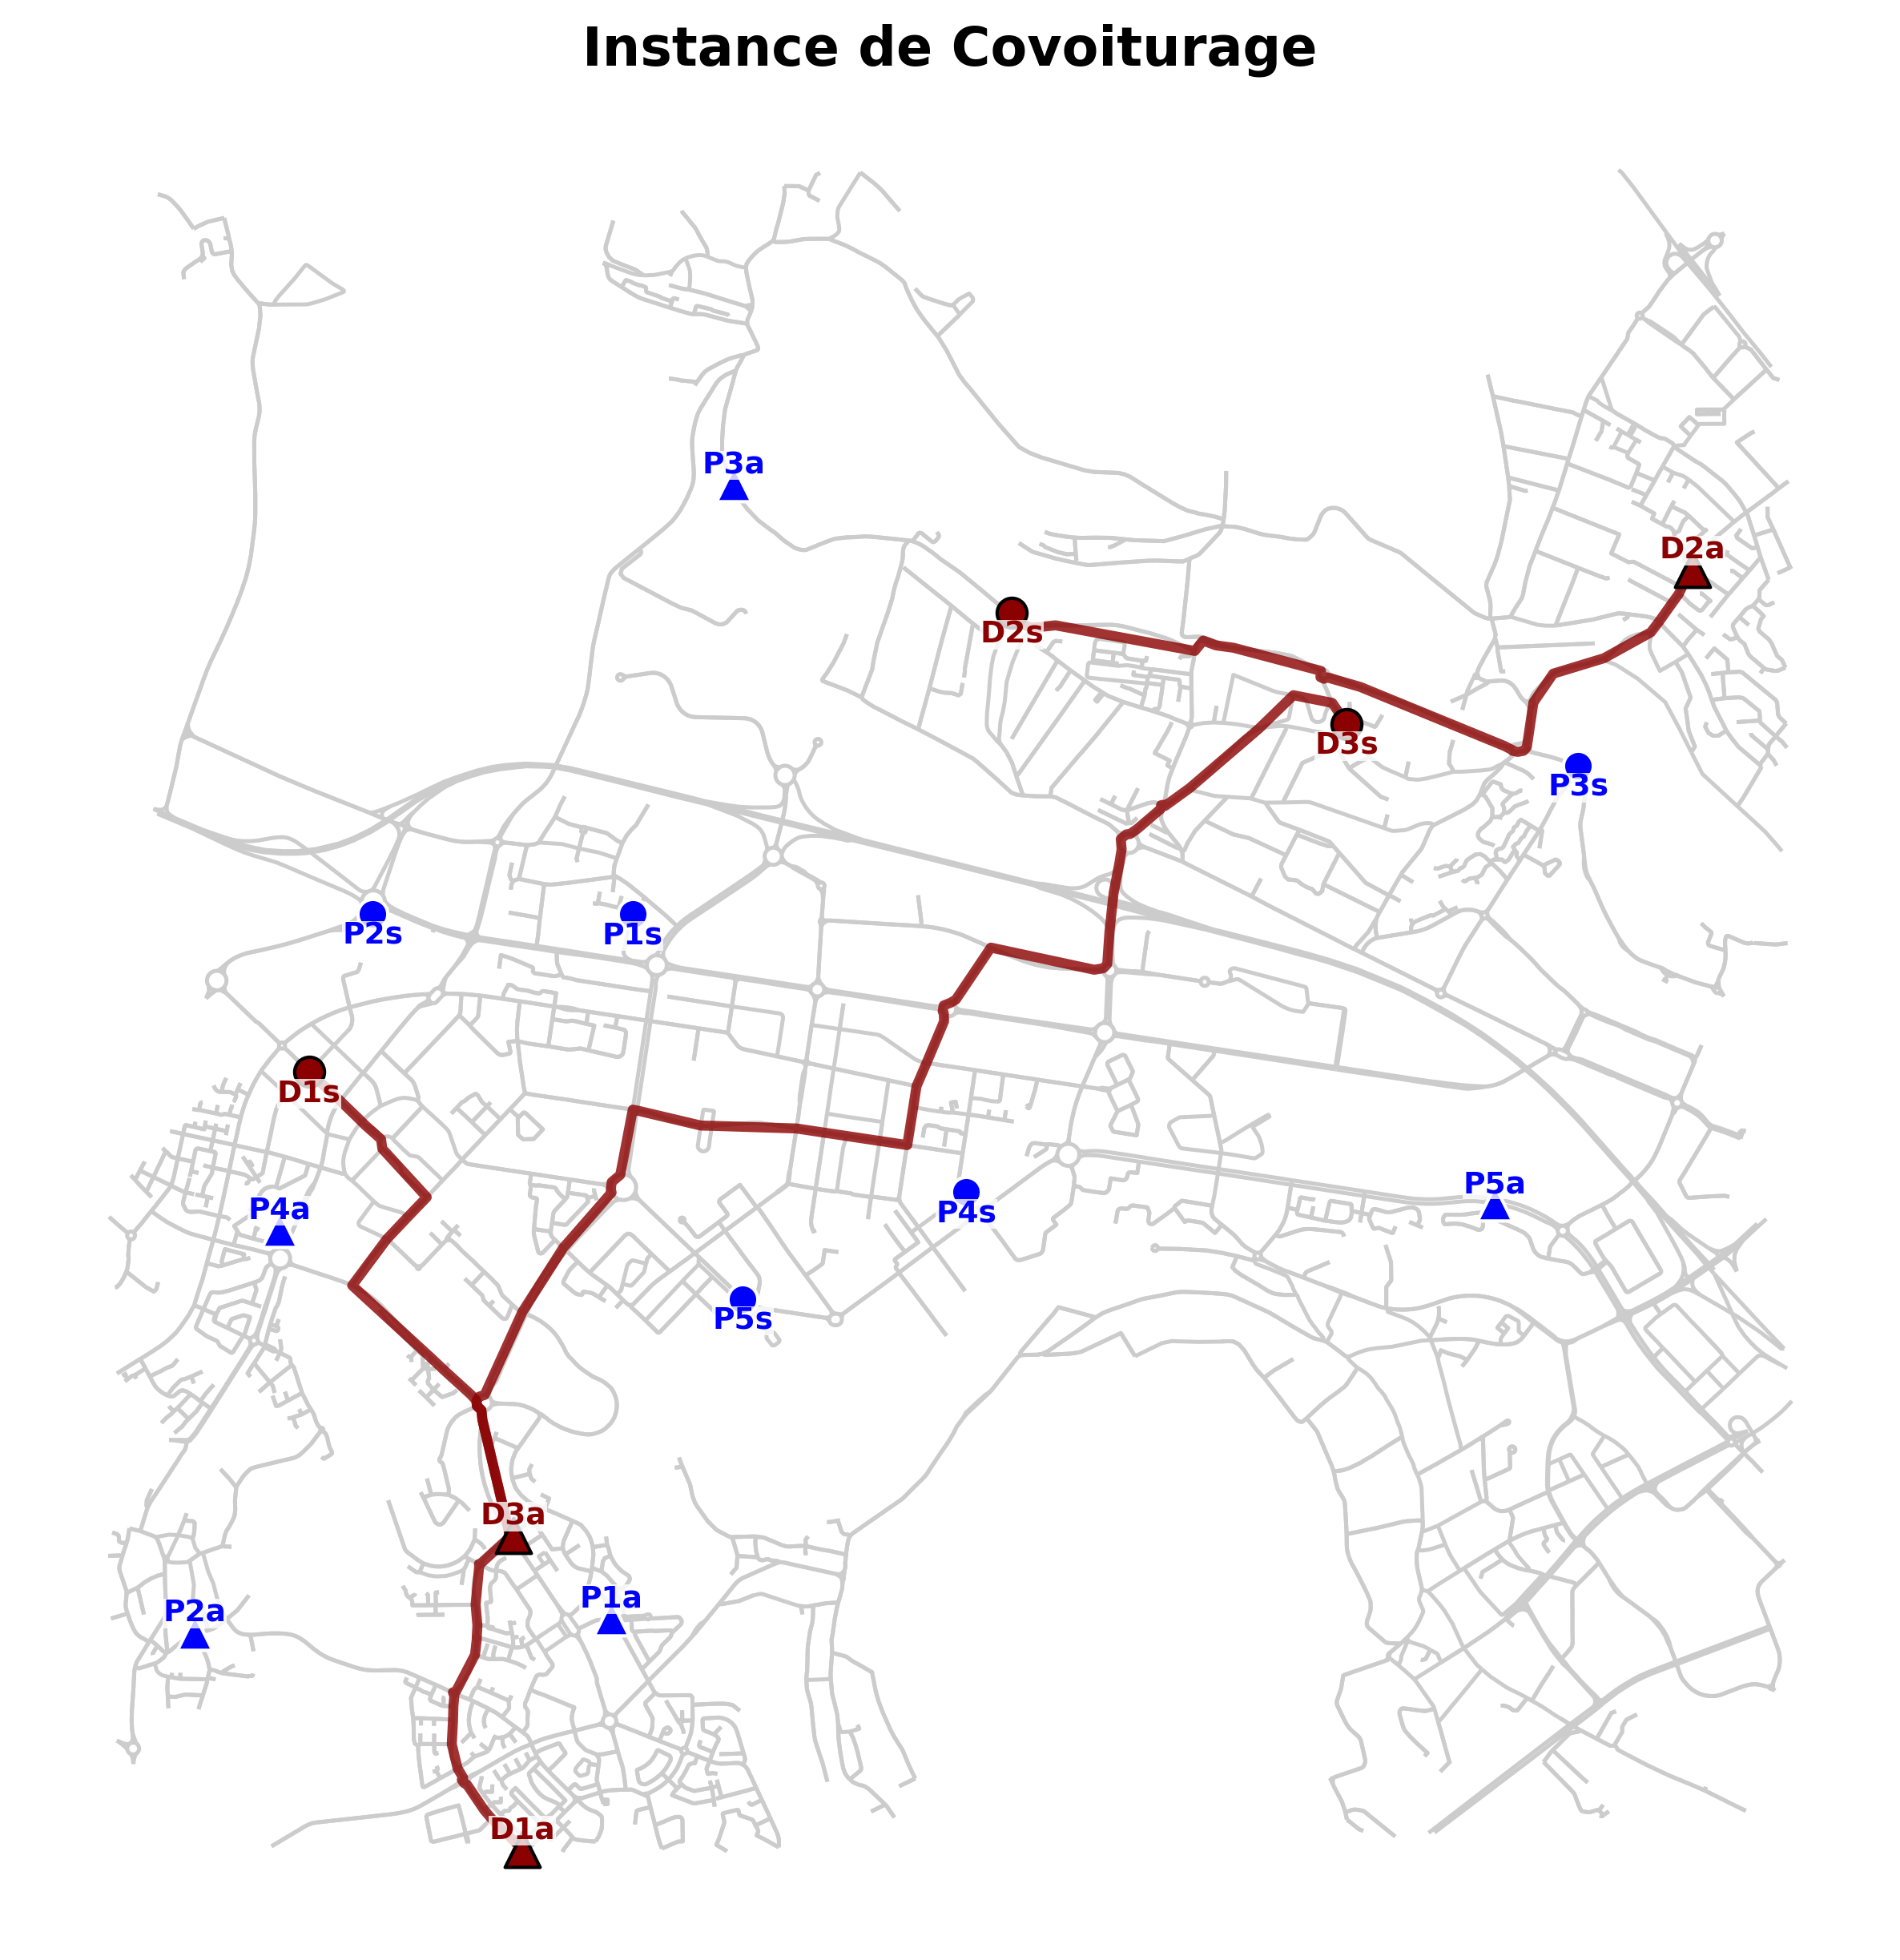
\includegraphics[width=0.7\textwidth]{map_covoiturage.png}
    \caption{Spatial representation of the road network and agents (Passengers in blue, Drivers in red) in Cergy.}
    \label{fig:reseau_cergy}
\end{figure}

\section{Definition of Concepts and Variables}

The modeling approach is dynamic. The assignment (or \textit{matching}) is defined as a function evolving over time.

\subsection{Agents and Time Interval}

The problem involves two types of agents:

\begin{itemize}
    \item $P = \{p_1, ..., p_n\}$, the set of passengers.
    \item $D = \{d_1, ..., d_k\}$, the set of real drivers.
\end{itemize}

To model the walking alternative, we introduce a set of ``phantom'' vehicles,
$F = \{f_1, ..., f_n\}$, one for each passenger.
The extended set of vehicles is denoted by: $D' = D \cup F$.

Matching is performed over a discretized time interval $T$:

\begin{itemize}
    \item Let $t_0$ denote the initial observation time of the problem.
    \item Let $\Delta t$ denote a predefined time step (e.g., 1 minute).
    \item The time interval is then defined as:
\end{itemize}
\[
T=\{t_0,t_0+\Delta t,t_0+2\Delta t,\ldots,t_F\},
\]
where $t_F$ denotes the final time of the problem.

By convention, all temporal variables defined in this model
($t_j^h$, $t_j^*$, $t_{d_i}^{max\_pickup}$, etc.) belong to $T$, while durations (denoted $\Delta t$) are assumed to be multiples of the time step.

\subsection{Temporal Definitions}

For each passenger $p_j$, we define the following temporal variables:

\begin{itemize}
    \item $t_j^h$ : departure time of passenger $p_j$ from home.
    \item $t_{i,j}^m$ : meeting time between passenger $p_j$ and driver $d_i$.
    \item $tt_{i,j}^{wo}$ : walking time required for passenger $p_j$ to reach the pickup point with driver $d_i$ (access time).
    \item $tt_{i,j}^{wd}$ : walking time required for passenger $p_j$ to reach the final destination from the drop-off point of driver $d_i$ (egress time).
    \item $tt_{i,j}^{c}$ : total ridesharing travel time for passenger $p_j$ with driver $d_i$.
    \item $tt_j^{M}$ : total walking time if passenger $p_j$ decides to walk to the destination.
    \item $t_j^*$ : desired arrival time of passenger $p_j$.
    \item $ta_j$ : actual arrival time at destination of passenger $p_j$.
\end{itemize}

\subsection{The Matching Function $\mu$}

Matching is defined as an application $\mu$ that, for each instant $t \in T$, associates an agent with a subset of other agents:

$$
\mu: T \times (P \cup D') \to \mathcal{P}(P \cup D')
$$

This function must satisfy the following consistency rules for all
$t \in T$, $p_j \in P$, and $d_i \in D'$:

\begin{enumerate}
    \item \textbf{Driver Perspective:}
    The image of a driver is the set of passengers carried at time $t$:

$$
\mu(t,d_i)\subseteq P
\quad\text{and}\quad
|\mu(t,d_i)|<q_i
$$

where $q_i$ is the total vehicle capacity of driver $d_i$ (including the driver).

Moreover, $\mu(t,d_i)$ must be a set of mutually compatible passengers.

For a phantom vehicle $f_j$, capacity is defined as:

$$
q_j=2
$$

(including the passenger).

    \item \textbf{Passenger Perspective:}
    The image of a passenger is the unique vehicle assigned to them:

$$
\mu(t',p_j)\subseteq D'
\quad\text{and}\quad
|\mu(t',p_j)|=1,
\quad \forall t' \geq t_j^h
$$

If $t<t_j^h$, the passenger is not yet active in the system and:

$$
\mu(t,p_j)=\emptyset.
$$

Furthermore, if $t\geq t_j^h$ and $\mu(t,p_j)\neq\{f_j\}$, then:

$$
\mu(t,p_j)\subset D.
$$

    \item \textbf{Consistency Condition:}
    A passenger $p_j$ belongs to the set of driver $d_i$ if and only if that passenger is assigned to that driver:

$$
p_j\in\mu(t,d_i)
\iff
\mu(t,p_j)=\{d_i\}
$$

\end{enumerate}

\section{Schedule Delay Cost (SDC): Analysis of Possible Functional Forms}

The Schedule Delay Cost (SDC) measures the disutility associated with the difference between actual arrival time ($ta_j$) and desired arrival time ($t_j^*$). Several formulations are possible depending on the behavioral assumptions retained.

\subsection{Symmetric Linear Model}

$$
SDC(ta_j,t_j^*)=\alpha |t_j^*-ta_j|
$$

Early arrival and late arrival are penalized equally.

\subsection{Quadratic Model}

$$
SDC(ta_j,t_j^*)=\alpha (t_j^*-ta_j)^2
$$

This specification heavily penalizes large deviations from the desired arrival time.

\subsection{Asymmetric Linear Model}

$$
SDC(ta_j,t_j^*)=
\beta (t_j^*-ta_j)^+
+
\gamma (ta_j-t_j^*)^+
$$

Typically, one assumes:

$$
\gamma>\alpha>\beta
$$

since being late is generally more costly (e.g., lost productivity, missed appointments) than arriving early (passive waiting time).

\subsection{Model with Fixed Late Arrival Penalty}

$$
SDC(ta_j,t_j^*)=
\beta (t_j^*-ta_j)^+
+
\gamma (ta_j-t_j^*)^+
+
\theta \mathbf 1_{ta_j>t_j^*}
$$

where $\theta$ is a fixed cost incurred whenever arrival occurs after the desired arrival time, independently of the duration of lateness.

\section{Analytical Definition of Costs}

Unlike previous static formulations in which costs were represented through a static matrix $C_{i,j}$, costs are here defined as dynamic functions depending on time and the agents involved. The objective is to capture more precisely the various components of the disutility associated with an assignment.

We distinguish three main types of costs:

\begin{itemize}
    \item ridesharing cost,
    \item walking cost,
    \item compatibility cost.
\end{itemize}

\subsection{Ridesharing Cost $C^c(t,d_i,p_j)$}

This cost represents the disutility incurred by passenger $p_j$ when assigned to vehicle $d_i$ at time $t$. It integrates travel time and punctuality considerations.

$$
\begin{aligned}
C^c(t,d_i,p_j)
&=
\alpha^c tt_{i,j}^c
+
SDC(t,ta_j,t_j^*)
\\
&\quad
+
\alpha^M
\left(
tt_{i,j}^{wo}
+
tt_{i,j}^{wd}
\right)
\end{aligned}
$$

where:

\begin{itemize}
    \item $tt_{i,j}^c$ is the total ridesharing travel time for passenger $p_j$ with driver $d_i$;

    \item $SDC(t,ta_j,t_j^*)$ is the schedule delay cost associated with passenger $p_j$, measuring dissatisfaction due to deviation between actual arrival time $ta_j$ and desired arrival time $t_j^*$;

    \item $tt_{i,j}^{wo}$ and $tt_{i,j}^{wd}$ denote respectively access walking time and egress walking time;

    \item $\alpha^c$ and $\alpha^M$ are unit cost coefficients for motorized transportation and walking.
\end{itemize}

\subsection{Walking Cost $C^M(t,p_j)$}

This cost is incurred when passenger $p_j$ chooses not to rideshare and instead uses the phantom vehicle $f_j$, implying that the passenger walks to the destination.

$$
C^M(t,p_j)=
\alpha^M tt_j^M
+
SDC(t,ta_j,t_j^*)
$$

\footnote{
The inclusion of SDC reflects the potential mismatch between walking speed and passenger scheduling constraints: lateness becomes unavoidable whenever $t_j^h+tt_j^M>t_j^*$.
}

where:

\begin{itemize}
    \item $tt_j^M$ is the total walking time to destination;

    \item $\alpha^M$ is the weighting coefficient associated with walking.
\end{itemize}

\subsection{Compatibility Cost $C^{comp}(t,d_i,p_j,O(t,d_i))$}

This additional cost captures the ``social disutility'' or friction associated with assigning an additional passenger $p_j$ to vehicle $d_i$ when the latter already contains a set of occupants. It reflects the need for social harmony among individuals sharing the same vehicle.

We define $O(t,d_i)$ as the set of occupants of vehicle $d_i$ at time $t$, including the driver $d_i$ and all passengers currently on board.

The compatibility cost $C^{comp}$ may be modeled in several ways.

\begin{itemize}

    \item \textbf{Binary Approach:}
    A high (possibly infinite) cost is incurred whenever passenger $p_j$ is incompatible with at least one occupant $x\in O(t,d_i)$:

$$
C^{comp}(t,d_i,p_j,O(t,d_i))
=
\begin{cases}
\infty
&
\text{if }\exists x\in O(t,d_i)
\text{ such that }(p_j,x)\text{ incompatible}
\\
0
&
\text{otherwise}
\end{cases}
$$

This corresponds to a clique condition where all members must be mutually compatible.

    \item \textbf{Continuous Approach:}
    Compatibility cost may alternatively be represented as the sum of pairwise incompatibility penalties:

$$
C^{comp}(t,d_i,p_j,O(t,d_i))
=
\sum_{x\in O(t,d_i)}
\text{penalty}(p_j,x)
$$

where $\text{penalty}(\cdot,\cdot)$ returns a positive value in case of incompatibility and zero otherwise.

\end{itemize}

In this model, we adopt the binary approach for strong compatibility constraints by assigning an infinite cost whenever incompatibility is detected.

The detailed incompatibility criteria (social preferences, behavioral preferences, etc.) are treated as exogenous input parameters of the model.

The final optimization objective is to minimize the sum of these costs over all assignments throughout the full time horizon $T$.


\section{Decentralized Modeling: Agent Decision Process}

This section formalizes the individual decision-making process of passengers. In this decentralized model, each passenger $p_j$ solves their own cost minimization problem at every decision time $t \in T$.

\subsection{Feasible Option Set}

Let $\Phi(t,p_j)\subseteq D'$ denote the set of admissible transportation options for passenger $p_j$ at time $t$. A vehicle $d_i$ (real or phantom) belongs to $\Phi(t,p_j)$ if and only if it satisfies all technical, temporal, and social feasibility constraints:

\begin{enumerate}

    \item \textbf{Capacity Constraint:}

$$
|O(t,d_i)\cap P|+1<q_i
$$

where $O(t,d_i)$ denotes the set of occupants of vehicle $d_i$ at time $t$, and $q_i$ its total capacity.

    \item \textbf{Temporal Feasibility:}

$$
\begin{cases}
t_{i,j}^m \geq t_j^h+tt_{i,j}^{wo}
\\
t_{i,j}^m \leq t_{d_i}^{max\_pickup}
\\
ta_j \leq t_j^*+\Delta t_j^{tolerance}
\end{cases}
$$

where:

\begin{itemize}
    \item $t_{i,j}^m$ and $ta_j$ denote estimated pickup and arrival times;

    \item $tt_{i,j}^{wo}$ is the walking time required to reach the pickup point;

    \item $t_{d_i}^{max\_pickup}$ is the latest admissible pickup time imposed by the driver's fixed route;

    \item $\Delta t_j^{tolerance}$ is the maximum delay tolerated by passenger $p_j$.
\end{itemize}

    \item \textbf{Social Compatibility Constraint:}

$$
C^{comp}(t,d_i,p_j,O(t,d_i))<\infty
$$

\end{enumerate}

\subsection{Individual Cost Minimization Problem and Preferences}

Each passenger $p_j$ chooses (or is assigned) a departure time $t_j^h\in T$ representing their initial availability. At decision time $t=t_j^h$, passenger $p_j$ seeks to minimize their total cost function $TC$ among all available options.

This rational behavior defines a \textbf{preference relation} $\succ_j$ over the admissible option set $\Phi(t,p_j)$. For two vehicles $d_1,d_2\in\Phi(t,p_j)$, passenger $p_j$ prefers $d_1$ over $d_2$ whenever the associated cost is lower:

$$
d_1\succ_j d_2
\iff
TC(t,p_j,d_1)<TC(t,p_j,d_2)
$$

The total individual cost function $TC$ is defined as:

$$
TC(t,p_j,d_i)=
\begin{cases}
C^c(t,d_i,p_j)
+
C^{comp}(t,d_i,p_j,O(t,d_i))
&
\text{if }d_i\in D
\\
C^M(t,p_j)
&
\text{if }d_i=f_j
\end{cases}
$$

This formulation ensures that each agent behaves rationally by ranking options according to their own utility while respecting the operational constraints and limits of the ridesharing system.

These preference lists form the basis of the matching algorithm.


\section{Objective: Search for a Stable Matching}

Within this decentralized modeling framework, the primary objective is to determine a \textbf{stable matching} over time.

\subsection{Matching Stability}

A matching $\mu^*$ is said to be stable if, for each passenger $p_j$ at their departure time $t=t_j^h$, the assignment constitutes a \textbf{stable equilibrium}. This means that there exists no \textbf{blocking pair} $(p_j,d_k)$ compatible with the system that would have an incentive to form outside the current matching.

More formally, a matching $\mu^*$ is stable if, for every passenger $p_j$ who would prefer a driver $d_k$ over their assigned driver $d_i^*=\mu^*(t_j^h,p_j)$, driver $d_k$ satisfies one of the following conditions:

\begin{enumerate}

    \item Driver $d_k$ is already at full capacity and prefers each of their currently assigned passengers over $p_j$;

    \item Driver $d_k$ is incompatible with $p_j$ (or one of the current occupants is incompatible with $p_j$), making the assignment infeasible:

$$
C^{comp}=\infty
$$

\end{enumerate}

This condition guarantees that, at that precise decision instant, no passenger has either the incentive or the possibility to deviate toward another option.

System stability is therefore intrinsically linked to the social cohesion of the groups formed.

Within this dynamic framework, once the matching is established at $t_j^h$, the passenger is considered committed to their trip.

A passenger remains unmatched (assigned to their phantom vehicle $f_j$) only if:

\begin{itemize}
    \item no compatible ridesharing option exists at time $t_j^h$, or

    \item the walking cost $C^M$ is lower than all real ridesharing alternatives available in $\Phi(t_j^h,p_j)$.
\end{itemize}

\subsection{Efficiency and Global Performance}

The secondary objective is to evaluate the quality of the resulting equilibrium relative to a theoretical global optimum.

To do so, the global efficiency of the system is measured through the sum of passenger costs over the full time horizon $T$:

$$
Z_{system}
=
\sum_{t\in T}
\sum_{\{p_j\in P\mid t_j^h=t\}}
TC\left(t,p_j,\mu^*(t,p_j)\right)
$$

Comparing this global cost resulting from decentralized individual decisions with the theoretical optimum of a centralized planner makes it possible to quantify the performance loss (or efficiency gap) of the decentralized system.


\section{Resolution Algorithm: Adapted Gale--Shapley Procedure}

To determine a stable matching at a given time $t$, we use an adaptation of the Gale--Shapley deferred acceptance algorithm, extended to the \textit{many-to-one} setting (multiple passengers per vehicle).

\subsection{Construction of Preference Lists}

The algorithm relies on the existence of preference rankings established by each agent:

\begin{itemize}

    \item \textbf{Passenger Preferences:}
    Each passenger $p_j$ ranks admissible vehicles $d_i\in\Phi(t,p_j)$ in increasing order of their total individual cost $TC(t,p_j,d_i)$.

    Their phantom vehicle $f_j$ is included in this ranking and represents the acceptability threshold beyond which ridesharing becomes less attractive than walking.

    \item \textbf{Driver Preferences:}
    Each driver $d_i$ ranks potential passengers according to a \textbf{proximity criterion}. A passenger is preferred if located spatially closer to the driver's fixed route, thereby minimizing the indirect cost of pickup.

\end{itemize}

\subsection{Algorithmic Procedure}

The process is iterated until stability is reached:

\begin{enumerate}

    \item \textbf{Proposal Phase:}
    Each passenger $p_j$ becoming available at time $t$ (i.e., such that $t=t_j^h$) proposes to the most preferred vehicle in their list $\Phi(t,p_j)$ that has not yet rejected them.

    \item \textbf{Deferred Acceptance Phase:}
    Each driver $d_i$ receives incoming proposals and temporarily accepts the best-ranked passengers according to their preference ordering, up to vehicle capacity $q_i$.

    All remaining passengers are rejected.

    \item \textbf{Termination:}
    The algorithm stops when no passenger has additional proposals to make.

    Passengers who fail to obtain a real driver are assigned to their phantom vehicle $f_j$.

\end{enumerate}

This mechanism guarantees the existence of a stable matching in the sense of user equilibrium.

\subsection{Stability Theorem and Proof}

To guarantee mathematical stability of the matching in this dynamic setting, we impose the following fundamental assumptions:

\begin{enumerate}

    \item \textbf{Single-Hop Assumption:}
    Each passenger $p_j$ may be assigned to one and only one vehicle $d_i\in D$ (or to their phantom vehicle $f_j$) for the entirety of their trip.

    \item \textbf{Irreversible Commitment Assumption:}
    Once matched at departure time $t_j^h$, the passenger is considered committed.

    They may neither revise their decision nor be reallocated at later times $t>t_j^h$.

    \item \textbf{Fixed Route Assumption for Drivers:}
    Each driver $d_i$ follows a predefined and invariant route.

    Ridesharing is only permitted if pickup and drop-off occur along this route (or within acceptable detour limits).

    \item \textbf{Local Perfect Information Assumption:}
    At each time step $t$, the system possesses exhaustive knowledge of:

$$
P_{active}(t)
$$

and the residual capacity of all vehicles.

\end{enumerate}

\textbf{Theorem 1 (Existence and Stability).}
Under the preceding assumptions, for every instance of the dynamic ridesharing problem defined at time $t$, there exists at least one stable matching $\mu^*(t,\cdot)$ in the Gale--Shapley sense (absence of compatible blocking pairs).

\textbf{Proof.}
The proof relies on the deferred acceptance mechanism previously described.

Suppose, by contradiction, that after completion of the matching procedure there exists a blocking pair $(p_j,d_k)$ such that passenger $p_j$ prefers driver $d_k$ to their final assignment, and driver $d_k$ prefers $p_j$ to at least one currently assigned passenger (or has remaining capacity).

\begin{enumerate}

    \item By the proposal rule, each passenger proposes to drivers in decreasing order of preference.

    \item Since $p_j$ prefers $d_k$ to their assigned driver, $p_j$ must necessarily have proposed to $d_k$ before being accepted by their final driver.

    \item If $p_j$ is not matched with $d_k$ at termination, then driver $d_k$ must have rejected them (either immediately or after later replacement).

    \item A driver rejects a passenger only if capacity is filled with passengers whom the driver strictly prefers.

    \item Therefore, at termination, driver $d_k$ must be full and all assigned passengers must rank above $p_j$ in the driver's preference ordering.

\end{enumerate}

This contradicts the initial assumption of a blocking pair.

Hence no blocking pair can exist, and the resulting matching is stable.


\subsection{Dynamic Algorithm Pseudo-Code}

The matching algorithm is executed iteratively over the entire time interval $T$ in order to account for the progressive arrival of passengers.

\begin{itemize}
    \item[] \textbf{For each time step $t\in T$:}

    \begin{enumerate}

        \item \textbf{Identification of New Passengers:}

$$
P_{active}(t)=\{p_j\in P\mid t=t_j^h\}
$$

        \item \textbf{Update of Available Capacities:}

        For each driver $d_i\in D$, the residual capacity $q_i(t)$ is computed by subtracting the number of passengers already present in the vehicle (matched during previous time steps and whose trip has not yet ended).

        \item \textbf{Local Stable Matching (Gale--Shapley):}

        Apply Gale--Shapley from $P_{active}(t)$ to $D'$ using residual capacities $q_i(t)$:

        \begin{itemize}

            \item passengers rank options according to $TC$;

            \item drivers rank candidates according to proximity;

            \item deferred acceptance is repeated until stability is achieved.

        \end{itemize}

        \item \textbf{Update of State $\mu^*(t,\cdot)$:}

        Newly established assignments are recorded and matched passengers are removed from the candidate pool for future time steps.

    \end{enumerate}

\end{itemize}

\section{Discussion and Perspectives: Toward a Multi-Hop Model}

The modeling framework presented in this document provides a stable and robust matching mechanism for simple ridesharing trips. However, the attainment of this stability relies on restrictive assumptions that limit the global optimality of the system.

\subsection{Limitations of the Current Model}

The main limitations identified are linked to the rigidity of the decision process:

\begin{itemize}

    \item \textbf{Absence of Transfers:}
    The Single-Hop assumption prevents passengers from using multiple successive vehicles.

    This penalizes long-distance trips when no single driver covers the full required path.

    \item \textbf{Early Commitment:}
    The irreversible commitment assumption prevents any renegotiation during the trip.

    A passenger dropped at an intermediate point is forced to complete the remainder of the trip on foot, even if a more advantageous ridesharing opportunity arises afterward.

\end{itemize}

\subsection{Perspective: Multi-Hop Extension}

To overcome these limitations, a natural extension of this work consists in modeling the problem as a \textbf{multi-hop matching problem}. In this framework, the Gale--Shapley algorithm would no longer be applied solely at the initial departure time $t_j^h$, but recursively throughout the trip.

\textbf{Extension Principle:}

Whenever a passenger is dropped off by a first driver $d_1$ at time

$$
t=t_{1,j}^m+tt_{1,j}^c,
$$

they are reintroduced into the active passenger set:

$$
P_{active}(t).
$$

Their new departure time becomes:

$$
t_j^h=t_{1,j}^m+tt_{1,j}^c,
$$

and their origin is updated to their current drop-off location.

Their preference list is then dynamically recomputed for the remaining segment of the trip toward the final destination.

This approach transforms the matching problem into a \textbf{dynamic path-search problem} over a ridesharing opportunity network, opening the way to substantially improved systemic efficiency.

However, this comes at the cost of increased algorithmic complexity and requires more sophisticated management of transfer times and temporal coordination.
\end{document}
